%!TEX program = lualatex
%!TEX options = --shell-escape

\documentclass[aspectratio=169]{beamer}

\usetheme{oxford}
\usefonttheme[onlymath]{serif}

\setsansfont{FoundrySterling-Book}[
  BoldFont=FoundrySterling-Bold,
  ItalicFont = FoundrySterling-BookItalic,
  SmallCapsFont = FoundrySterling-BookExpert
]

\usepackage{booktabs}

\title{\Huge RL in NL\\\Large A little reinforcement learning example in NetLogo}
\date{\scriptsize June 4\textsuperscript{th} 2020}
\author{Nicolas Payette}
\institute{%
  
\includegraphics[height=1cm]{geog-brand-pos}%
  
\includegraphics[height=1cm]{ox_brand_cmyk_pos.eps}
}

\newcommand\lbl[1]{\text{\footnotesize\begin{tabular}{@{}c@{}}#1\end{tabular}}}

\begin{document}

\maketitle

\begin{frame}[wide]{Use reinforcement learning when...}
  \huge
  \begin{tcolorbox}[halign=flush center]
    Agents' \hl{actions} generate \hl{rewards} from the \hl{environment} over time.
  \end{tcolorbox}
  \vfill\Large
  \begin{description}[But it's trial-and-error search:]
    \item [It can handle delayed reward:] when actions taken \hl{now} can affect \hl{future} rewards.
    \item [But it's trial-and-error search:] agents have to try different actions to evaluate their effects.
  \end{description}
\end{frame}

\begin{frame}{Agent-environment interaction in RL}
  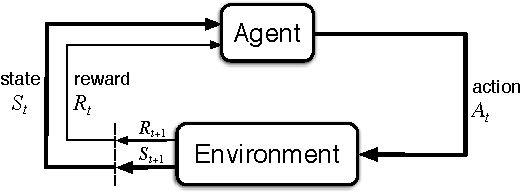
\includegraphics[width=\textwidth]{agent-env-interaction}
  \vfill\hfill\small Sutton \& Barto (2017) \emph{Reinforcement Learning: An Introduction}
\end{frame}

\begin{frame}{Temporal difference learning: TD(0)}
  \large Actions are chosen using an \hl{${\boldmath\Large\epsilon}$-greedy} policy:
  \begin{equation*}
    A \gets
    \begin{cases}
      \textrm{a random action},                 & \textrm{with probability } \epsilon\\
      \textrm{the action that maximizes }V(S'), & \textrm{otherwise}
    \end{cases}
  \end{equation*}
  \begin{columns}
    \begin{column}{0.65\textwidth}
      Agents must learn the value of the possible \hl{states}:
      \begin{equation*}
        V(S) \gets V(S) + \alpha\bigg(\,\overbrace{R + \gamma V(S') - V(S)}^{\lbl{TD error}}\,\bigg)
      \end{equation*}
    \end{column}
    \pause
    \begin{column}{0.3\textwidth}
      \begin{tcolorbox}[title=Constraint, left=1mm, right=1mm, halign=flush left]
         Only works if the agent has a model of the environment:
         if it knows which action will bring about which state.
      \end{tcolorbox}
    \end{column}
  \end{columns}
\end{frame}

\begin{frame}{The Q function}
  \Huge
  \begin{equation*}
    Q: State \times Action \to Value
  \end{equation*}
  \vfill~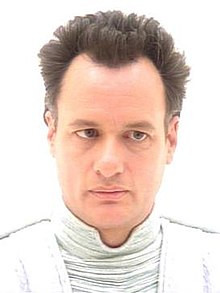
\includegraphics[width=0.15\textwidth]{q.jpg}
\end{frame}

\begin{frame}
  \vfill
  \hl{\Large SARSA} (on-policy -- when you care about reward \emph{while} learning):
  \begin{equation*}
    \small
    Q(S,A) \gets
      \underbrace{Q(S,A)}_{\lbl{old\\value}}
      +
      \underbrace{\alpha}_{\lbl{learning\\rate}}
      \bigg(
      \overbrace{
        \underbrace{R}_{\lbl{reward}}
        +
        \underbrace{\gamma}_{\lbl{discount\\factor}}
        \cdot\:
        \textcolor{gray}{\underbrace{\textcolor{OxfordBlue}{Q(S', A')}}_{\lbl{\hl{value of next}\\\hl{action taken}}}}
      -\:
      Q(S,A)
      }^{\lbl{TD error}}
      \bigg)
  \end{equation*}
  \vfill
  \hl{\Large Q-Learning} (off-policy -- when you just care about finding the optimal policy):
  \begin{equation*}
    \small
    Q(S,A) \gets
      \underbrace{Q(S,A)}_{\lbl{old\\value}}
      +
      \underbrace{\alpha}_{\lbl{learning\\rate}}
      \bigg(
      \overbrace{
        \underbrace{R}_{\lbl{reward}}
        +
        \underbrace{\gamma}_{\lbl{discount\\factor}}
        \cdot\:
        \textcolor{gray}{\underbrace{\textcolor{OxfordBlue}{\max_{a}Q(S', a)}}_{\lbl{\hl{value of best}\\\hl{possible action}}}}%
      -\:
      Q(S,A)
      }^{\lbl{TD error}}
      \bigg)
  \end{equation*}
  \vfill
  \begin{tcolorbox}
    Still $\epsilon$-greedy, but this time we choose the action with the best Q-value.
  \end{tcolorbox}
\end{frame}

\begin{frame}{Example: the windy grid world}
  \centering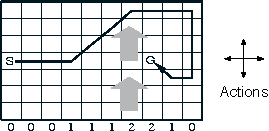
\includegraphics[width=\textwidth]{windy_grid_world.pdf}
\end{frame}

\begin{frame}{Sounds like a good candidate for a NetLogo model?}
  \vfill
  \centering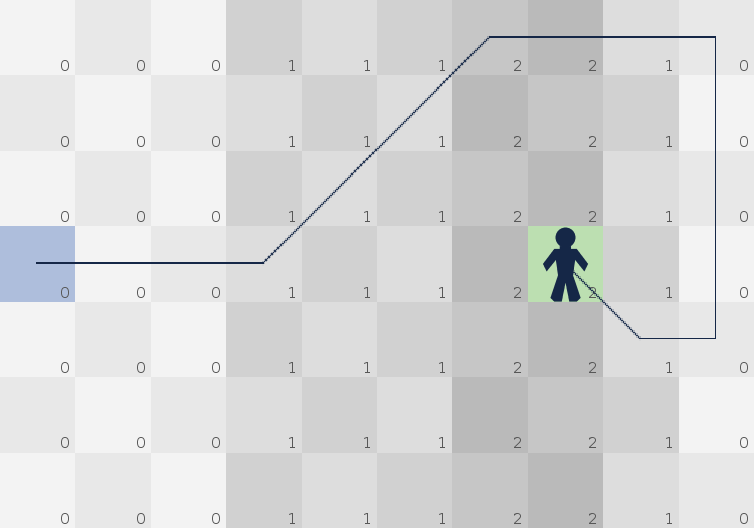
\includegraphics[height=0.8\textheight]{rl_view}
  \vfill
\end{frame}

\end{document}
